\documentclass[12pt, oneside, openany]{article}
\usepackage[utf8]{inputenc}
\usepackage{polski}
\renewcommand*{\figurename}{Rys.}
\usepackage{graphicx}
\usepackage{float}
\usepackage{geometry}
\geometry{
	left=25mm,
	right=25mm,%
	bindingoffset=10mm, 
	top=25mm, 
	bottom=25mm}
\title{
	Eksploracyjna analiza danych \\
	Światowy program szczepień przeciwko COVID-19
}
\author{
	Marek Grudkowski 156587
	\\
	Kamil Kaczmarkiewicz 171701
}

\begin{document}

\maketitle

\section{Ogólny opis danych}

Zbiór danych dotyczy aktualnego postępu poszczególnych państw w szczepieniach przeciwko COVID-19. Zawiera on informacje pochodzące prawie ze wszystkich krajów na świecie podzielone na poszczególne dni. Program szczepień przeciwko COVID to w dobie pandemii niezwykle gorący temat. Naszym zdaniem warto się na nim skupić, gdyż może zawierać wiele ukrytych informacji, które mogą przydać się w walce z pandemią i przyspieszyć sam proces szczepień. 

\section{Cel eksploracji i kryteria sukcesu}

\newpage

\section{Charakterystyka zbioru danych}
Zbiór danych na stan dnia pisania tego sprawozdania zawiera ponad 13300 przykładów. Dane aktualizowane są zazwyczaj każdego dnia i pochodzą z wielu różnych źródeł. Zazwyczaj są nimi organy krajowe lub lokalne, czy międzynarodowe organizacje. Dla każdego przykładu podane jest źródło i jego adres internetowy, co daje możliwość weryfikacji w przypadku jakichkolwiek wątpliwości co do poprawności danych. Dane zapisane są w jednym pliku w formacie csv i podzielone są na następujące kolumny:
\begin{itemize}
\item \textbf{country} - kraj, dla którego podawane są informacje o szczepieniu, atrybut nominalny w postaci ciągu znaków
\item \textbf{iso\_code} - kod ISO dla danego kraju, atrybut nominalny w postaci ciągu znaków
\item \textbf{date} - data wprowadzenia danych, atrybut nominalny opisujący datę
\item \textbf{total\_vaccinations} - bezwzględna liczba wszystkich szczepień ochronnych w danym kraju, atrybut numeryczny (liczba naturalna)
\item \textbf{people\_vaccinated} - liczba osób która otrzymała szczepionkę (przy dwóch dawkach liczona jest $\times2$), atrybut numeryczny (liczba naturalna)
\item \textbf{people\_fully\_vaccinated} -  liczba osób, które otrzymały cały zestaw szczepień, atrybut numeryczny (liczba naturalna)
\item \textbf{daily\_vaccinations\_raw} - dla danej pozycji liczba szczepień dla tej daty/kraju, atrybut numeryczny (liczba naturalna)
\item \textbf{daily\_vaccinations} - dla danej pozycji liczba szczepień dla tej daty/kraju, atrybut numeryczny (liczba naturalna)
\item \textbf{total\_vaccinations\_per\_hundred} - stosunek liczby szczepień do całkowitej liczby ludności danego dnia w kraju, atrybut numeryczny wyrażany w procentach
\item \textbf{people\_vaccinated\_per\_hundred} - stosunek liczby osób zaszczepionych do całkowitej liczby ludności danego dnia w kraju, atrybut numeryczny wyrażany w procentach
\item \textbf{people\_fully\_vaccinated\_per\_hundred} - stosunek liczby osób uodpornionych do całkowitej liczby ludności danego dnia w kraju, atrybut numeryczny wyrażany w procentach
\item \textbf{daily\_vaccinations\_per\_million} - stosunek między liczbą szczepień a całkowitą liczbą ludności na bieżący dzień w kraju, dodania liczba rzeczywista
\item \textbf{vaccines} - rodzaje szczepionek wykorzystanych w danym kraju, atrybut nominalny, ciągi znaków rozdzielone ukośnikiem
\item \textbf{source\_name} - źródło informacji, atrybut nominalny, ciąg znaków
\item \textbf{source\_website} - strona internetowa źródła informacji, atrybut nominalny, ciąg znaków
\end{itemize}


\section{Wyniki eksploracyjnej analizy danych}



Podczas analizowania danych pierwszym etapem, było sprawdzenie w jakiej ilości występują wartości zerowe lub \textit{NaN}. Ku naszemu zaskoczeniu przykładów z takimi wartościami było naprawdę dużo. Wyniki tej operacji poniżej. 

\begin{center}
\begin{table}[h]
\begin{tabular}{|l|c|}
\hline
\multicolumn{1}{|c|}{\textbf{Atrybut}} & \textbf{Brakujące wartości} \\ \hline
country                                & 0                           \\ \hline
iso\_code                              & 0                           \\ \hline
date                                   & 0                           \\ \hline
total vaccinations                     & 5390                        \\ \hline
people vaccinated                      & 6069                        \\ \hline
people fully vaccinated                & 8069                        \\ \hline
daily vaccinations raw                 & 6685                        \\ \hline
daily vaccinations                     & 226                         \\ \hline
total vaccinations per hundred         & 5390                        \\ \hline
people vaccinated per hundred          & 6069                        \\ \hline
people fully vaccinated per hundred    & 8069                        \\ \hline
daily vaccinations per million         & 226                         \\ \hline
vaccines                               & 0                           \\ \hline
source name                            & 0                           \\ \hline
source website                         & 0                           \\ \hline
\end{tabular}
\end{table}
\end{center}

W tabeli można zauważyć, że liczba brakujących wartości dla atrybutów takich jak \textit{people\_fully\_vaccinated\_per\_hundred} i \textit{people\_vaccinated\_per\_hundred} są takie same jak dla \textit{people\_fully\_vaccinated} i \textit{people\_vaccinated}. Na 9 atrybutów, w których występują brakujące dane, 8 z nich tworzy właśnie takie pary. Jedynym \textit{samotnym} atrybutem jest \textit{daily\_vaccinations\_raw}. Jego nazwa wskazuje, że mógłby mieć powiązanie z atrybutem \textit{daily\_vaccinations}, ale żeby to stwierdzić, trzeba wyliczyć korelację między tymi atrybutami porzucając te przykłady, w których występują braki. 


Kolejnym krokiem było utworzenie diagramu, który wizualizuje współczynnik korelacji pomiędzy poszczególnymi atrybutami. Widać na nim, że są one podzielone na dwie podgrupy, w których występują silne zależności między atrybutami. Pierwszą z nich zaklasyfikowaliśmy jako dane bezwzględne i zawiera atrybuty, które opisują bezwzględne wartości liczbowe np. liczba zaszczepionych osób. Druga grupa dotyczy atrybutów, których wartości podawane są w procentach np. liczba osób w pełni zaszczepionych na sto. 

\begin{center}
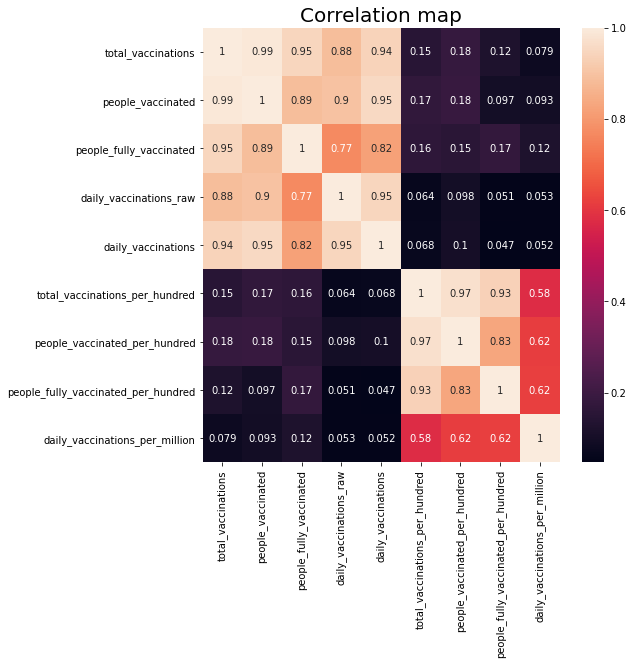
\includegraphics[scale=0.7]
{../img/corelation.png} 
\end{center}

Mimo ładnego podziału zbioru atrybutów na dwie grupy, pojawiło się pytanie - dlaczego zauważamy bardzo niską korelacją pomiędzy atrybutami, które powinny być ze sobą powiązane w dużym stopniu. Chodzi tutaj na przykład o sumę ludzi w pełni zaszczepionych oraz procent ludzi w pełni zaszczepionych na sto. Być może ma to związek z tym, że powyższy diagram przedstawia dane dotyczące całego świata, a pojedyncze przykłady dotyczą konkretnych państw. By to sprawdzić zrealizowaliśmy podobny wykres, ale opisujący  tylko zbiór przykładów z takich państw jak Niemcy, USA i Polska.

\begin{center}
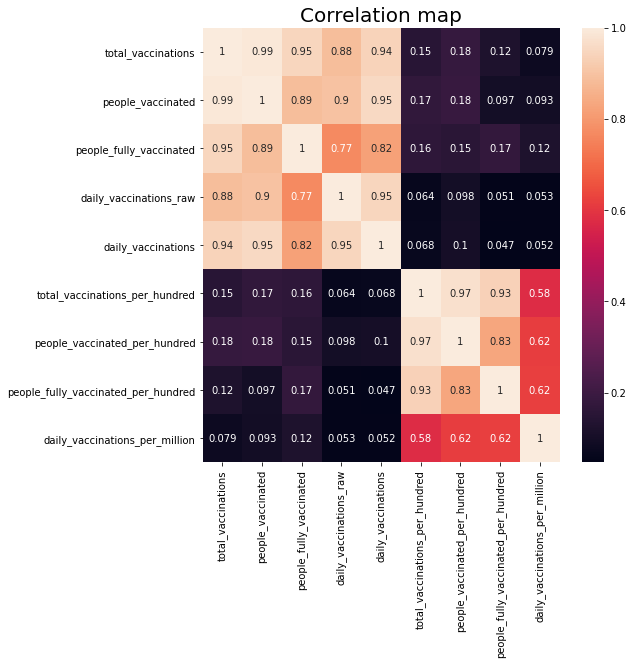
\includegraphics[scale=0.7]
{../img/corelation.png} 
\end{center}


Rozkłady wartości dla atrybutów 

rozkłady wartości atrybutów, korelacje pomiędzy wartościami atrybutów
wstępne ustalenia dotyczące zawartości zbioru 
\section{Uwagi dotyczące jakości danych}
dane brakujące, punkty oddalone, dane niespójne, dane niezrozumiałe,
\section{Opis wyników eksploracji}

w odniesieniu do celów eksploracji, czy dane są wystarczające, ewentualna rewizja celów

\end{document}
